\documentclass[a4paper]{jpconf}

\usepackage{graphicx}

\usepackage{hyperref}

\usepackage[sort&compress,numbers]{natbib}

%\usepackage{cite}

\usepackage{amsmath}
\usepackage{amssymb}
\usepackage{bm}

\newcommand{\maestroex}{{\sffamily MAESTROeX}}
\newcommand{\castro}{{\sffamily Castro}}
\newcommand{\starkiller}{{\sffamily StarKiller}}
\newcommand{\starlord}{{\sffamily StarLord}}
\newcommand{\nyx}{{\sffamily Nyx}}
\newcommand{\amrex}{{\sffamily AMReX}}
\newcommand{\vode}{{\sffamily VODE}}

\newcommand{\Uc}{{\,\bm{\mathcal{U}}}}
\newcommand{\Adv}[1]{{\left [\boldsymbol{\mathcal{A}} \left(#1\right)\right]}}
\newcommand{\Advt}[1]{{\left [\mathcal{\tilde{A}} \left(#1\right)\right]}}
\newcommand{\Advs}[1]{\boldsymbol{\mathcal{A}} \left(#1\right)}

\newcommand{\isot}[2]{$^{#2}\mathrm{#1}$}
\newcommand{\avg}[1]{{\left \langle #1 \right \rangle}}
\newcommand{\Rbs}[1]{{\bf R} \left ( #1 \right )}
\newcommand{\Ic}{\bm{\mathcal{I}}}

\newcommand{\gcc}{\mathrm{g~cm^{-3} }}
\newcommand{\cms}{\mathrm{cm~s^{-1} }}



\newcommand{\cpp}{C\nolinebreak\hspace{-.05em}\raisebox{.4ex}{\tiny\bf +}\nolinebreak\hspace{-.10em}\raisebox{.4ex}{\tiny\bf +}}

\usepackage{color}
\setlength{\marginparwidth}{0.75in}
\newcommand{\MarginPar}[1]{\marginpar{\vskip-\baselineskip\raggedright\tiny\sffamily\hrule\smallskip{\color{red}#1}\par\smallskip\hrule}}

\newcommand{\apj}{Astrophysical Journal}
\newcommand{\aap}{Astronomy and Astrophysics}
\newcommand{\mnras}{Monthly Notices of the Royal Astronomical Society}
\newcommand{\prd}{Physical Review D}
\newcommand{\apjs}{Astrophysical Journal Supplement}

\begin{document}

\title{The Castro AMR Simulation Code: Current and Future Developments}

\author{M. Zingale$^1$,
        A.~S.~Almgren$^2$,
        M.~Barrios Sazo$^1$,
        J.~B. Bell$^4$,
        K.~Eiden$^1$,
        A.~Harpole$^1$,
        M.~P. Katz$^3$,
        A.~J. Nonaka$^2$,
        D.~E. Willcox$^2$, and
        W. Zhang$^2$}

\address{$^1$Department of Physics and Astronomy, Stony Brook
  University, Stony Brook, NY 11794-3800 USA}

\address{$^2$Center for Computational Sciences and Engineering,
  Lawrence Berkeley National Lab, Berkeley, CA 94720 USA}

\address{$^3$NVIDIA Corporation, 2788 San Tomas Expressway,
  Santa Clara, CA, 95050 USA}

\ead{michael.zingale@stonybrook.edu}

\begin{abstract}
We describe the \castro\ astrophysics simulation code, focusing on the
recent developments in coupling hydrodynamics and reactions and describing
upcoming developments.
\end{abstract}



\section{Introduction}

The \castro\ astrophysical simulation code~\cite{castro} is designed
for modeling problems in nuclear astrophysics, with the ability to
accurately capture the interplay between hydrodynamics, reactions,
gravity, and radiation in stars with complex equations of state.
Since \castro\ was first developed, there have been a number of
enhancements to the code base, expanding its applicability to a new
range of scientific problems.  The most active development presently
focuses on new methods of time integration, with better coupling of
physical processes, and GPU performance.  Here we discuss some of
these features.

\castro\ has been applied to models of Type Ia supernovae,
core-collapse supernovae, pair-instability supernovae, exoplanet
atmospheres, and most recently X-ray bursts (see, e.g.,
\cite{castro-ccsne,castro-pairinstability,polin:2019,wdmergerI} for
some example science applications).  A common challenge in modeling
these events is the range of length and timescales involved.  To
capture length scales, \castro\ uses adaptive mesh refinement, through
the \amrex\ library~\cite{amrex_joss}.  This allows us to focus the
computational effort of regions where burning or the flow is
important.  To address the range of timescales involved in
astrophysical explosions, we have developed a low Mach number
hydrodynamics code, \maestroex~\cite{maestroex}, built on the same
framework as \castro, that can model the subsonic convection that
often precedes explosive events.  Both codes are open source and
freely available on
github\footnote{\url{https://github.com/AMReX-Astro/}}.

In the next sections, we discuss \castro's new approach to coupling
hydrodynamics and reactions and our efforts on performance portavbility.
We illustrate these new developments with our X-ray burst problem.

\section{Modeling Reactive Flow}

In modeling stellar explosions, it is often the case that the
hydrodynamics method and the nuclear reaction network require
different timesteps in order to produce stable and accurate models.
For the stiff nuclear reactions we encounter in stars, implicit ODE
method are often used together with operator splitting to evolve the
nuclear reactions separately from the hydrodynamics.  In the limit of
small timesteps, the two processes are well-coupled together, but
these conditions are not always met in simulations.  The recent focus
in \castro\ has been on high-fidelity simulations of reactive flow.
In \cite{castro:sdc} we introduced a new time integration strategy,
spectral deferred corrections (SDC), that eliminates the coupling
error introduced by commonly used operator splitting techniques (see
the discussion in \cite{astronum:2018} for a graphical illustration of
splitting error).

The SDC algorithm used in \castro\ follows the ideas of
\cite{dutt:2000,minion:2003}, and uses low order explicit advection
and implicit reaction updates in a correction equation that when
applied iteratively achieves high-order time-accuracy.  In an operator
split implementation, reaction and burning proceed without knowing
about the other process.  In contrast, the update in the SDC
formulation explicitly couples the processes together.  In \castro\ we
consider reactions and hydrodynamics, and write our conservative
system as:
\begin{equation}
\Uc_t = \Advs{\Uc} + \Rbs{\Uc}
\end{equation}
where $\Uc$ is the vector of conserved quantities, $\Advs{\Uc}$ is the
advective term (the divergence of the hydrodynamic fluxes along with
hydrodynamic sources), and $\Rbs{\Uc}$ are the reactive source terms.
The update is done at specific temporal nodes, the number of location
of which are picked to give the desired temporal accuracy.  The update
from one time node $m$ to $m+1$ appears as:
    \begin{align}
      \label{eq:sdc:general}
      \avg{\Uc}^{{m+1},(k+1)} = \avg{\Uc}^{m,(k+1)}
            &+ \delta t_m \left [ \avg{\Advs{\Uc}}^{m,(k+1)} - \avg{\Advs{\Uc}}^{m,(k)} \right ] \nonumber \\
            &+ \delta t_m \left [ \avg{\Rbs{\Uc}}^{{m+1},(k+1)} - \avg{\Rbs{\Uc}}^{{m+1},(k)} \right ] \nonumber \\
            &+ \int_{t^m}^{t^{m+1}} dt  \left (\avg{\Advs{\Uc}}^{(k)} + \avg{\Rbs{\Uc}}^{(k)}\right)
   \end{align}
We use a finite-volume formalism, so $\avg{\Uc}$ is the average of the
conserved state in a zone, $\avg{\Advs{\Uc}}^m$ is the average
advective term in a zone at time $t^m$, and $\avg{\Rbs{\Uc}}^{k+1}$ is
the average of the reactive source at time $t^{m+1}$.  The second
superscript on each term, $(k)$ or $(k+1)$, is the iteration.  This
update is an implicit equation for the new state,
$\avg{\Uc}^{{m+1},(k+1)}$.  The last term in the update is an integral
over the sources constructed from the previous iteration's values at
each time node.  Each iteration of the SDC method increases the
temporal order of accuracy by one, up to the order of accuracy with
which the integral is constructed.  

\castro\ implements both a second-order method (using a trapezoid rule
for the integral) and fourth-order method in space and time (using a
Simpsons rule for the integral and the spatial reconstruction of
\cite{mccorquodalecolella}).  We demonstrated that \castro\ achieves
the expected convergence on a wide variety of problems in
\cite{castro:sdc}.  At the moment, the method is limited to single
levels, but work is underway to extend this methodology to AMR.  For
problems where burning is imprtant and can dominate the computational
expense, we expect these new SDC method will become the preferred
integration technique in the future.


\section{Performance Portability}

The original approach to parallelism in \castro\ was MPI + OpenMP,
with scaling on manycore architectures achieve using a tiling approach
to OpenMP~\cite{tiling}.  More recently we've ported \castro\ to GPUs
using CUDA, using the same computational kernels as the MPI + OpenMP
version.  This reuse keeps the code base managable---we don't need
separate kernels for each architecture---while allowing us to take
advantage of current and next generation supercomputers.  All of the
solvers needed to run our core science problems run on GPUs: the main
unsplit PPM hydrodynamics scheme~\cite{ppm,millercolella:2002}, self-gravity via multigrid with
isolated boundary conditions, thermal diffusion, and nuclear
reactions.  Our approach is to put the data on GPUs and then run all
of the kernels on the GPUs, minimizing data movement.  This has given
us enormous speed-ups.

\begin{figure}[t]
\centering
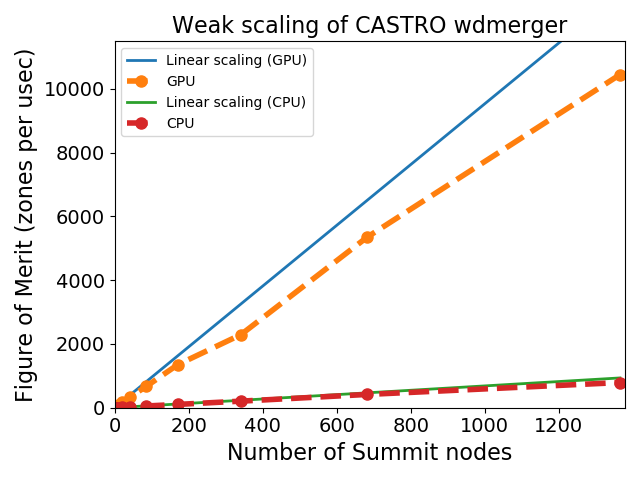
\includegraphics[width=0.8\linewidth]{wdmerger_gpu}
\caption{\label{fig:gpu} blah}
\end{figure}

\section{Example Application}

The SDC approach was demonstrated in \cite{castro:sdc} through a large
suite of convergence tests and a thermonuclear flame problem.  

We've run XRB on GPUs and with SDC


\section{Future Developments}

The development of SDC in \castro\ continues, with the current focus
on modeling detonations.  Reactions in astrophysical detonations are
especially stiff and challenging to model when the ash state reaches
nuclear statistical equilibrium.  We are exploring different
quadrature schemes for the integral in Equation~\ref{eq:sdc} to model
detonations in the SDC framework.  We are also working on extending
the SDC integration methodology to adaptive mesh refinement with
subcycling in time.

To complement the existing suite of hydrodynamics solver in \castro,
an MHD solver is under development and expected to be merged into the
main branch soon.  We will use the experiences learned with the
\castro\ hydrodynamics solver to port this solver to GPUs and fit into
the SDC framework.

All of these developments fit into our goal of modeling XRBs.


\ack The work at Stony Brook was supported by DOE/Office of Nuclear
Physics grant DE-FG02-87ER40317 and contract 7418390 with Lawrence
Berkeley National Laboratory as part of the Exascale Compute Project
ExaStar collaboration.  This research was supported by the Exascale
Computing Project (17-SC-20-SC), a collaborative effort of the
U.S. Department of Energy Office of Science and the National Nuclear
Security Administration.  The work at LBNL was supported by the DOE
Office of Advanced Scientific Computing Research under Contract No,
DE-AC02-05CH11231.  An award of computer time was provided by the
Innovative and Novel Computational Impact on Theory and Experiment
(INCITE) program. This research used resources of the Oak Ridge
Leadership Computing Facility at the Oak Ridge National Laboratory,
which is supported by the Office of Science of the U.S. Department of
Energy under Contract No.\ DE-AC05-00OR22725.  This research used
resources of the National Energy Research Scientific Computing Center,
which is supported by the Office of Science of the U.S. Department of
Energy under Contract No.\ DE-AC02-05CH11231.  Visualizations were
done using yt~\cite{yt}.  This research has made use of NASA's
Astrophysics Data System Bibliographic Services.


%\section*{References}

\bibliographystyle{iopart-num}
\bibliography{ws}


\end{document}
